\documentclass{beamer}
\usepackage[utf8]{inputenc}

\usepackage{fourier} %font utopia imported
\usetheme{Madrid}
\usecolortheme{default}

%------------------------------------------------------------
%This block of code defines the information to appear in the
%Title page
\title[An FMI-Based initialization plugin for INTO-CPS Maestro 2] %optional
{An FMI-Based initialization plugin for INTO-CPS Maestro 2}
\date{\today}
\usepackage{booktabs}
\usepackage{natbib}
\usepackage{tikz}
\usepackage{multicol}
\usepackage{hyperref}
\usepackage{pgfplots}
\usepackage{listings}
\usepackage{tikz}
\usepackage{environ}
\usepackage{filecontents}
\usepackage{verbatim}
\usepackage{graphicx}
\usepackage{amsfonts}
\usepackage{amsmath}
\usepackage{amssymb}
\usepackage{stmaryrd}
\usepackage{amstext}
\usepackage{semantic}
\hypersetup{
    colorlinks=true,
    linkcolor=red,
    filecolor=magenta,      
    urlcolor=cyan,
}
\definecolor{codegreen}{rgb}{0,0.6,0}
\definecolor{codegray}{rgb}{0.5,0.5,0.5}
\definecolor{codepurple}{rgb}{0.58,0,0.82}
\definecolor{backcolour}{rgb}{0.95,0.95,0.92}
\usefonttheme{serif} % <----------- HERE

\lstdefinestyle{mystyle}{
    backgroundcolor=\color{backcolour},   
    commentstyle=\color{codegreen},
    keywordstyle=\color{magenta},
    numberstyle=\tiny\color{codegray},
    stringstyle=\color{codepurple},
    basicstyle=\ttfamily\footnotesize,
    breakatwhitespace=false,         
    breaklines=true,                 
    captionpos=b,                    
    keepspaces=true,                 
    numbers=left,                    
    numbersep=5pt,                  
    showspaces=false,                
    showstringspaces=false,
    showtabs=false,                  
    tabsize=2
}

\lstset{style=mystyle}
\begin{filecontents*}{incorrect.csv}
a,b,c
0,0,0
0.008,-0.000313843,-0.0313843
0.016,-0.00125348,-0.125348
0.024,-0.00280998,-0.280998
0.032,-0.00496389,-0.496389
0.04,-0.00768499,-0.768499
0.048,-0.0109346,-1.09346
0.056,-0.014669,-1.4669
0.064,-0.0188426,-1.88426
0.072,-0.0234109,-2.34109
0.08,-0.0283315,-2.83315
0.088,-0.0335644,-3.35644
0.096,-0.0390719,-3.90719
0.104,-0.044817,-4.4817
0.112,-0.0507637,-5.07637
0.12,-0.0568755,-5.68755
0.128,-0.0631156,-6.31156
0.136,-0.0694474,-6.94474
0.144,-0.0758344,-7.58344
0.152,-0.0822408,-8.22408
0.16,-0.0886322,-8.86322
0.168,-0.0949758,-9.49758
0.176,-0.10124,-10.124
0.184,-0.107397,-10.7397
0.192,-0.113418,-11.3418
0.2,-0.119277,-11.9277
0.208,-0.124952,-12.4952
0.216,-0.130421,-13.0421
0.224,-0.135663,-13.5663
0.232,-0.140659,-14.0659
0.24,-0.145395,-14.5395
0.248,-0.149855,-14.9855
0.256,-0.154027,-15.4027
0.264,-0.157901,-15.7901
0.272,-0.161467,-16.1467
0.28,-0.164721,-16.4721
0.288,-0.167656,-16.7656
0.296,-0.170271,-17.0271
0.304,-0.172564,-17.2564
0.312,-0.174535,-17.4535
0.32,-0.176188,-17.6188
0.328,-0.177525,-17.7525
0.336,-0.178553,-17.8553
0.344,-0.179277,-17.9277
0.352,-0.179705,-17.9705
0.36,-0.179848,-17.9848
0.368,-0.179715,-17.9715
0.376,-0.179317,-17.9317
0.384,-0.178666,-17.8666
0.392,-0.177777,-17.7777
0.4,-0.176662,-17.6662
0.408,-0.175336,-17.5336
0.416,-0.173814,-17.3814
0.424,-0.172111,-17.2111
0.432,-0.170243,-17.0243
0.44,-0.168226,-16.8226
0.448,-0.166076,-16.6076
0.456,-0.16381,-16.381
0.464,-0.161443,-16.1443
0.472,-0.158991,-15.8991
0.48,-0.15647,-15.647
0.488,-0.153897,-15.3897
0.496,-0.151286,-15.1286
0.504,-0.148651,-14.8651
0.512,-0.146009,-14.6009
0.52,-0.143372,-14.3372
0.528,-0.140753,-14.0753
0.536,-0.138166,-13.8166
0.544,-0.135623,-13.5623
0.552,-0.133134,-13.3134
0.56,-0.130712,-13.0712
0.568,-0.128365,-12.8365
0.576,-0.126102,-12.6102
0.584,-0.123933,-12.3933
0.592,-0.121865,-12.1865
0.6,-0.119904,-11.9904
0.608,-0.118056,-11.8056
0.616,-0.116327,-11.6327
0.624,-0.114721,-11.4721
0.632,-0.113241,-11.3241
0.64,-0.11189,-11.189
0.648,-0.110671,-11.0671
0.656,-0.109583,-10.9583
0.664,-0.108629,-10.8629
0.672,-0.107807,-10.7807
0.68,-0.107117,-10.7117
0.688,-0.106557,-10.6557
0.696,-0.106125,-10.6125
0.704,-0.105818,-10.5818
0.712,-0.105634,-10.5634
0.72,-0.105568,-10.5568
0.728,-0.105616,-10.5616
0.736,-0.105773,-10.5773
0.744,-0.106035,-10.6035
0.752,-0.106396,-10.6396
0.76,-0.106851,-10.6851
0.768,-0.107392,-10.7392
0.776,-0.108016,-10.8016
0.784,-0.108714,-10.8714
0.792,-0.10948,-10.948
0.8,-0.110309,-11.0309
0.808,-0.111193,-11.1193
0.816,-0.112125,-11.2125
0.824,-0.113099,-11.3099
0.832,-0.114109,-11.4109
0.84,-0.115148,-11.5148
0.848,-0.116208,-11.6208
0.856,-0.117285,-11.7285
0.864,-0.118371,-11.8371
0.872,-0.119462,-11.9462
0.88,-0.12055,-12.055
0.888,-0.121632,-12.1632
0.896,-0.1227,-12.27
0.904,-0.123751,-12.3751
0.912,-0.124779,-12.4779
0.92,-0.12578,-12.578
0.928,-0.126751,-12.6751
0.936,-0.127687,-12.7687
0.944,-0.128584,-12.8584
0.952,-0.12944,-12.944
0.96,-0.130252,-13.0252
0.968,-0.131018,-13.1018
0.976,-0.131734,-13.1734
0.984,-0.1324,-13.24
0.992,-0.133014,-13.3014
1,-0.133575,-13.3575
1.008,-0.134082,-13.4082
1.016,-0.134534,-13.4534
1.024,-0.134931,-13.4931
1.032,-0.135274,-13.5274
1.04,-0.135562,-13.5562
1.048,-0.135796,-13.5796
1.056,-0.135978,-13.5978
1.064,-0.136108,-13.6108
1.072,-0.136187,-13.6187
1.08,-0.136217,-13.6217
1.088,-0.1362,-13.62
1.096,-0.136138,-13.6138
1.104,-0.136033,-13.6033
1.112,-0.135886,-13.5886
1.12,-0.135701,-13.5701
1.128,-0.13548,-13.548
1.136,-0.135225,-13.5225
1.144,-0.134939,-13.4939
1.152,-0.134624,-13.4624
1.16,-0.134284,-13.4284
1.168,-0.133921,-13.3921
1.176,-0.133537,-13.3537
1.184,-0.133136,-13.3136
1.192,-0.132721,-13.2721
1.2,-0.132293,-13.2293
1.208,-0.131856,-13.1856
1.216,-0.131412,-13.1412
1.224,-0.130964,-13.0964
1.232,-0.130514,-13.0514
1.24,-0.130065,-13.0065
1.248,-0.129619,-12.9619
1.256,-0.129177,-12.9177
1.264,-0.128743,-12.8743
1.272,-0.128318,-12.8318
1.28,-0.127904,-12.7904
1.288,-0.127503,-12.7503
1.296,-0.127116,-12.7116
1.304,-0.126745,-12.6745
1.312,-0.12639,-12.639
1.32,-0.126054,-12.6054
1.328,-0.125737,-12.5737
1.336,-0.12544,-12.544
1.344,-0.125164,-12.5164
1.352,-0.124909,-12.4909
1.36,-0.124676,-12.4676
1.368,-0.124466,-12.4466
1.376,-0.124278,-12.4278
1.384,-0.124112,-12.4112
1.392,-0.12397,-12.397
1.4,-0.123849,-12.3849
1.408,-0.123751,-12.3751
1.416,-0.123675,-12.3675
1.424,-0.12362,-12.362
1.432,-0.123586,-12.3586
1.44,-0.123572,-12.3572
1.448,-0.123577,-12.3577
1.456,-0.123602,-12.3602
1.464,-0.123644,-12.3644
1.472,-0.123703,-12.3703
1.48,-0.123779,-12.3779
1.488,-0.123869,-12.3869
1.496,-0.123974,-12.3974
1.504,-0.124091,-12.4091
1.512,-0.12422,-12.422
1.52,-0.12436,-12.436
1.528,-0.124509,-12.4509
1.536,-0.124667,-12.4667
1.544,-0.124832,-12.4832
1.552,-0.125003,-12.5003
1.56,-0.125179,-12.5179
1.568,-0.125359,-12.5359
1.576,-0.125542,-12.5542
1.584,-0.125727,-12.5727
1.592,-0.125912,-12.5912
1.6,-0.126098,-12.6098
1.608,-0.126282,-12.6282
1.616,-0.126464,-12.6464
1.624,-0.126644,-12.6644
1.632,-0.126819,-12.6819
1.64,-0.12699,-12.699
1.648,-0.127156,-12.7156
1.656,-0.127316,-12.7316
1.664,-0.12747,-12.747
1.672,-0.127617,-12.7617
1.68,-0.127756,-12.7756
1.688,-0.127887,-12.7887
1.696,-0.128011,-12.8011
1.704,-0.128125,-12.8125
1.712,-0.128231,-12.8231
1.72,-0.128327,-12.8327
1.728,-0.128415,-12.8415
1.736,-0.128493,-12.8493
1.744,-0.128562,-12.8562
1.752,-0.128621,-12.8621
1.76,-0.128672,-12.8672
1.768,-0.128713,-12.8713
1.776,-0.128745,-12.8745
1.784,-0.128768,-12.8768
1.792,-0.128783,-12.8783
1.8,-0.128789,-12.8789
1.808,-0.128787,-12.8787
1.816,-0.128778,-12.8778
1.824,-0.128761,-12.8761
1.832,-0.128736,-12.8736
1.84,-0.128706,-12.8706
1.848,-0.128669,-12.8669
1.856,-0.128626,-12.8626
1.864,-0.128578,-12.8578
1.872,-0.128525,-12.8525
1.88,-0.128467,-12.8467
1.888,-0.128406,-12.8406
1.896,-0.128341,-12.8341
1.904,-0.128273,-12.8273
1.912,-0.128203,-12.8203
1.92,-0.12813,-12.813
1.928,-0.128056,-12.8056
1.936,-0.12798,-12.798
1.944,-0.127904,-12.7904
1.952,-0.127827,-12.7827
1.96,-0.127751,-12.7751
1.968,-0.127675,-12.7675
1.976,-0.1276,-12.76
1.984,-0.127526,-12.7526
1.992,-0.127453,-12.7453
2,-0.127382,-12.7382
2.008,-0.127314,-12.7314
2.016,-0.127248,-12.7248
2.024,-0.127184,-12.7184
2.032,-0.127123,-12.7123
2.04,-0.127066,-12.7066
2.048,-0.127011,-12.7011
2.056,-0.12696,-12.696
2.064,-0.126913,-12.6913
2.072,-0.126869,-12.6869
2.08,-0.126829,-12.6829
2.088,-0.126793,-12.6793
2.096,-0.12676,-12.676
2.104,-0.126732,-12.6732
2.112,-0.126707,-12.6707
2.12,-0.126686,-12.6686
2.128,-0.126669,-12.6669
2.136,-0.126655,-12.6655
2.144,-0.126646,-12.6646
2.152,-0.126639,-12.6639
2.16,-0.126637,-12.6637
2.168,-0.126637,-12.6637
2.176,-0.126641,-12.6641
2.184,-0.126648,-12.6648
2.192,-0.126658,-12.6658
2.2,-0.12667,-12.667
2.208,-0.126685,-12.6685
2.216,-0.126703,-12.6703
2.224,-0.126723,-12.6723
2.232,-0.126744,-12.6744
2.24,-0.126768,-12.6768
2.248,-0.126793,-12.6793
2.256,-0.12682,-12.682
2.264,-0.126848,-12.6848
2.272,-0.126877,-12.6877
2.28,-0.126907,-12.6907
2.288,-0.126937,-12.6937
2.296,-0.126968,-12.6968
2.304,-0.127,-12.7
2.312,-0.127031,-12.7031
2.32,-0.127063,-12.7063
2.328,-0.127094,-12.7094
2.336,-0.127125,-12.7125
2.344,-0.127156,-12.7156
2.352,-0.127186,-12.7186
2.36,-0.127215,-12.7215
2.368,-0.127243,-12.7243
2.376,-0.127271,-12.7271
2.384,-0.127297,-12.7297
2.392,-0.127322,-12.7322
2.4,-0.127346,-12.7346
2.408,-0.127368,-12.7368
2.416,-0.127389,-12.7389
2.424,-0.127409,-12.7409
2.432,-0.127427,-12.7427
2.44,-0.127444,-12.7444
2.448,-0.127459,-12.7459
2.456,-0.127472,-12.7472
2.464,-0.127484,-12.7484
2.472,-0.127495,-12.7495
2.48,-0.127503,-12.7503
2.488,-0.127511,-12.7511
2.496,-0.127516,-12.7516
2.504,-0.12752,-12.752
2.512,-0.127523,-12.7523
2.52,-0.127524,-12.7524
2.528,-0.127524,-12.7524
2.536,-0.127522,-12.7522
2.544,-0.12752,-12.752
2.552,-0.127516,-12.7516
2.56,-0.127511,-12.7511
2.568,-0.127505,-12.7505
2.576,-0.127497,-12.7497
2.584,-0.127489,-12.7489
2.592,-0.12748,-12.748
2.6,-0.127471,-12.7471
2.608,-0.12746,-12.746
2.616,-0.127449,-12.7449
2.624,-0.127438,-12.7438
2.632,-0.127426,-12.7426
2.64,-0.127414,-12.7414
2.648,-0.127401,-12.7401
2.656,-0.127388,-12.7388
2.664,-0.127375,-12.7375
2.672,-0.127362,-12.7362
2.68,-0.127349,-12.7349
2.688,-0.127336,-12.7336
2.696,-0.127323,-12.7323
2.704,-0.127311,-12.7311
2.712,-0.127298,-12.7298
2.72,-0.127286,-12.7286
2.728,-0.127275,-12.7275
2.736,-0.127263,-12.7263
2.744,-0.127252,-12.7252
2.752,-0.127242,-12.7242
2.76,-0.127232,-12.7232
2.768,-0.127223,-12.7223
2.776,-0.127214,-12.7214
2.784,-0.127206,-12.7206
2.792,-0.127198,-12.7198
2.8,-0.127192,-12.7192
2.808,-0.127185,-12.7185
2.816,-0.12718,-12.718
2.824,-0.127175,-12.7175
2.832,-0.127171,-12.7171
2.84,-0.127167,-12.7167
2.848,-0.127164,-12.7164
2.856,-0.127162,-12.7162
2.864,-0.12716,-12.716
2.872,-0.127159,-12.7159
2.88,-0.127158,-12.7158
2.888,-0.127158,-12.7158
2.896,-0.127159,-12.7159
2.904,-0.12716,-12.716
2.912,-0.127162,-12.7162
2.92,-0.127164,-12.7164
2.928,-0.127166,-12.7166
2.936,-0.127169,-12.7169
2.944,-0.127172,-12.7172
2.952,-0.127176,-12.7176
2.96,-0.12718,-12.718
2.968,-0.127184,-12.7184
2.976,-0.127189,-12.7189
2.984,-0.127194,-12.7194
2.992,-0.127198,-12.7198
3,-0.127204,-12.7204
3.008,-0.127209,-12.7209
3.016,-0.127214,-12.7214
3.024,-0.127219,-12.7219
3.032,-0.127225,-12.7225
3.04,-0.12723,-12.723
3.048,-0.127235,-12.7235
3.056,-0.127241,-12.7241
3.064,-0.127246,-12.7246
3.072,-0.127251,-12.7251
3.08,-0.127256,-12.7256
3.088,-0.127261,-12.7261
3.096,-0.127266,-12.7266
3.104,-0.12727,-12.727
3.112,-0.127274,-12.7274
3.12,-0.127278,-12.7278
3.128,-0.127282,-12.7282
3.136,-0.127286,-12.7286
3.144,-0.127289,-12.7289
3.152,-0.127292,-12.7292
3.16,-0.127295,-12.7295
3.168,-0.127298,-12.7298
3.176,-0.1273,-12.73
3.184,-0.127302,-12.7302
3.192,-0.127304,-12.7304
3.2,-0.127305,-12.7305
3.208,-0.127307,-12.7307
3.216,-0.127308,-12.7308
3.224,-0.127308,-12.7308
3.232,-0.127309,-12.7309
3.24,-0.127309,-12.7309
3.248,-0.127309,-12.7309
3.256,-0.127309,-12.7309
3.264,-0.127308,-12.7308
3.272,-0.127308,-12.7308
3.28,-0.127307,-12.7307
3.288,-0.127306,-12.7306
3.296,-0.127305,-12.7305
3.304,-0.127303,-12.7303
3.312,-0.127302,-12.7302
3.32,-0.1273,-12.73
3.328,-0.127298,-12.7298
3.336,-0.127297,-12.7297
3.344,-0.127295,-12.7295
3.352,-0.127293,-12.7293
3.36,-0.12729,-12.729
3.368,-0.127288,-12.7288
3.376,-0.127286,-12.7286
3.384,-0.127284,-12.7284
3.392,-0.127282,-12.7282
3.4,-0.127279,-12.7279
3.408,-0.127277,-12.7277
3.416,-0.127275,-12.7275
3.424,-0.127273,-12.7273
3.432,-0.127271,-12.7271
3.44,-0.127269,-12.7269
3.448,-0.127267,-12.7267
3.456,-0.127265,-12.7265
3.464,-0.127263,-12.7263
3.472,-0.127261,-12.7261
3.48,-0.127259,-12.7259
3.488,-0.127258,-12.7258
3.496,-0.127256,-12.7256
3.504,-0.127255,-12.7255
3.512,-0.127254,-12.7254
3.52,-0.127252,-12.7252
3.528,-0.127251,-12.7251
3.536,-0.12725,-12.725
3.544,-0.127249,-12.7249
3.552,-0.127249,-12.7249
3.56,-0.127248,-12.7248
3.568,-0.127248,-12.7248
3.576,-0.127247,-12.7247
3.584,-0.127247,-12.7247
3.592,-0.127247,-12.7247
3.6,-0.127247,-12.7247
3.608,-0.127247,-12.7247
3.616,-0.127247,-12.7247
3.624,-0.127247,-12.7247
3.632,-0.127247,-12.7247
3.64,-0.127248,-12.7248
3.648,-0.127248,-12.7248
3.656,-0.127249,-12.7249
3.664,-0.127249,-12.7249
3.672,-0.12725,-12.725
3.68,-0.12725,-12.725
3.688,-0.127251,-12.7251
3.696,-0.127252,-12.7252
3.704,-0.127253,-12.7253
3.712,-0.127254,-12.7254
3.72,-0.127255,-12.7255
3.728,-0.127255,-12.7255
3.736,-0.127256,-12.7256
3.744,-0.127257,-12.7257
3.752,-0.127258,-12.7258
3.76,-0.127259,-12.7259
3.768,-0.12726,-12.726
3.776,-0.127261,-12.7261
3.784,-0.127262,-12.7262
3.792,-0.127263,-12.7263
3.8,-0.127264,-12.7264
3.808,-0.127264,-12.7264
3.816,-0.127265,-12.7265
3.824,-0.127266,-12.7266
3.832,-0.127267,-12.7267
3.84,-0.127267,-12.7267
3.848,-0.127268,-12.7268
3.856,-0.127269,-12.7269
3.864,-0.127269,-12.7269
3.872,-0.12727,-12.727
3.88,-0.12727,-12.727
3.888,-0.127271,-12.7271
3.896,-0.127271,-12.7271
3.904,-0.127271,-12.7271
3.912,-0.127272,-12.7272
3.92,-0.127272,-12.7272
3.928,-0.127272,-12.7272
3.936,-0.127272,-12.7272
3.944,-0.127273,-12.7273
3.952,-0.127273,-12.7273
3.96,-0.127273,-12.7273
3.968,-0.127273,-12.7273
3.976,-0.127273,-12.7273
3.984,-0.127273,-12.7273
3.992,-0.127272,-12.7272
4,-0.127272,-12.7272
4.008,-0.127272,-12.7272
\end{filecontents*}

\begin{filecontents*}{correct.csv}
a,b
0,-0.13
0.008,-0.13
0.016,-0.13
0.024,-0.13
0.032,-0.13
0.04,-0.13
0.048,-0.13
0.056,-0.13
0.064,-0.13
0.072,-0.13
0.08,-0.13
0.088,-0.13
0.096,-0.13
0.104,-0.13
0.112,-0.13
0.12,-0.13
0.128,-0.13
0.136,-0.13
0.144,-0.13
0.152,-0.13
0.16,-0.13
0.168,-0.13
0.176,-0.13
0.184,-0.13
0.192,-0.13
0.2,-0.13
0.208,-0.13
0.216,-0.13
0.224,-0.13
0.232,-0.13
0.24,-0.13
0.248,-0.13
0.256,-0.13
0.264,-0.13
0.272,-0.13
0.28,-0.13
0.288,-0.13
0.296,-0.13
0.304,-0.13
0.312,-0.13
0.32,-0.13
0.328,-0.13
0.336,-0.13
0.344,-0.13
0.352,-0.13
0.36,-0.13
0.368,-0.13
0.376,-0.13
0.384,-0.13
0.392,-0.13
0.4,-0.13
0.408,-0.13
0.416,-0.13
0.424,-0.13
0.432,-0.13
0.44,-0.13
0.448,-0.13
0.456,-0.13
0.464,-0.13
0.472,-0.13
0.48,-0.13
0.488,-0.13
0.496,-0.13
0.504,-0.13
0.512,-0.13
0.52,-0.13
0.528,-0.13
0.536,-0.13
0.544,-0.13
0.552,-0.13
0.56,-0.13
0.568,-0.13
0.576,-0.13
0.584,-0.13
0.592,-0.13
0.6,-0.13
0.608,-0.13
0.616,-0.13
0.624,-0.13
0.632,-0.13
0.64,-0.13
0.648,-0.13
0.656,-0.13
0.664,-0.13
0.672,-0.13
0.68,-0.13
0.688,-0.13
0.696,-0.13
0.704,-0.13
0.712,-0.13
0.72,-0.13
0.728,-0.13
0.736,-0.13
0.744,-0.13
0.752,-0.13
0.76,-0.13
0.768,-0.13
0.776,-0.13
0.784,-0.13
0.792,-0.13
0.8,-0.13
0.808,-0.13
0.816,-0.13
0.824,-0.13
0.832,-0.13
0.84,-0.13
0.848,-0.13
0.856,-0.13
0.864,-0.13
0.872,-0.13
0.88,-0.13
0.888,-0.13
0.896,-0.13
0.904,-0.13
0.912,-0.13
0.92,-0.13
0.928,-0.13
0.936,-0.13
0.944,-0.13
0.952,-0.13
0.96,-0.13
0.968,-0.13
0.976,-0.13
0.984,-0.13
0.992,-0.13
1,-0.13
1.008,-0.13
1.016,-0.13
1.024,-0.13
1.032,-0.13
1.04,-0.13
1.048,-0.13
1.056,-0.13
1.064,-0.13
1.072,-0.13
1.08,-0.13
1.088,-0.13
1.096,-0.13
1.104,-0.13
1.112,-0.13
1.12,-0.13
1.128,-0.13
1.136,-0.13
1.144,-0.13
1.152,-0.13
1.16,-0.13
1.168,-0.13
1.176,-0.13
1.184,-0.13
1.192,-0.13
1.2,-0.13
1.208,-0.13
1.216,-0.13
1.224,-0.13
1.232,-0.13
1.24,-0.13
1.248,-0.13
1.256,-0.13
1.264,-0.13
1.272,-0.13
1.28,-0.13
1.288,-0.13
1.296,-0.13
1.304,-0.13
1.312,-0.13
1.32,-0.13
1.328,-0.13
1.336,-0.13
1.344,-0.13
1.352,-0.13
1.36,-0.13
1.368,-0.13
1.376,-0.13
1.384,-0.13
1.392,-0.13
1.4,-0.13
1.408,-0.13
1.416,-0.13
1.424,-0.13
1.432,-0.13
1.44,-0.13
1.448,-0.13
1.456,-0.13
1.464,-0.13
1.472,-0.13
1.48,-0.13
1.488,-0.13
1.496,-0.13
1.504,-0.13
1.512,-0.13
1.52,-0.13
1.528,-0.13
1.536,-0.13
1.544,-0.13
1.552,-0.13
1.56,-0.13
1.568,-0.13
1.576,-0.13
1.584,-0.13
1.592,-0.13
1.6,-0.13
1.608,-0.13
1.616,-0.13
1.624,-0.13
1.632,-0.13
1.64,-0.13
1.648,-0.13
1.656,-0.13
1.664,-0.13
1.672,-0.13
1.68,-0.13
1.688,-0.13
1.696,-0.13
1.704,-0.13
1.712,-0.13
1.72,-0.13
1.728,-0.13
1.736,-0.13
1.744,-0.13
1.752,-0.13
1.76,-0.13
1.768,-0.13
1.776,-0.13
1.784,-0.13
1.792,-0.13
1.8,-0.13
1.808,-0.13
1.816,-0.13
1.824,-0.13
1.832,-0.13
1.84,-0.13
1.848,-0.13
1.856,-0.13
1.864,-0.13
1.872,-0.13
1.88,-0.13
1.888,-0.13
1.896,-0.13
1.904,-0.13
1.912,-0.13
1.92,-0.13
1.928,-0.13
1.936,-0.13
1.944,-0.13
1.952,-0.13
1.96,-0.13
1.968,-0.13
1.976,-0.13
1.984,-0.13
1.992,-0.13
2,-0.13
2.008,-0.13
2.016,-0.13
2.024,-0.13
2.032,-0.13
2.04,-0.13
2.048,-0.13
2.056,-0.13
2.064,-0.13
2.072,-0.13
2.08,-0.13
2.088,-0.13
2.096,-0.13
2.104,-0.13
2.112,-0.13
2.12,-0.13
2.128,-0.13
2.136,-0.13
2.144,-0.13
2.152,-0.13
2.16,-0.13
2.168,-0.13
2.176,-0.13
2.184,-0.13
2.192,-0.13
2.2,-0.13
2.208,-0.13
2.216,-0.13
2.224,-0.13
2.232,-0.13
2.24,-0.13
2.248,-0.13
2.256,-0.13
2.264,-0.13
2.272,-0.13
2.28,-0.13
2.288,-0.13
2.296,-0.13
2.304,-0.13
2.312,-0.13
2.32,-0.13
2.328,-0.13
2.336,-0.13
2.344,-0.13
2.352,-0.13
2.36,-0.13
2.368,-0.13
2.376,-0.13
2.384,-0.13
2.392,-0.13
2.4,-0.13
2.408,-0.13
2.416,-0.13
2.424,-0.13
2.432,-0.13
2.44,-0.13
2.448,-0.13
2.456,-0.13
2.464,-0.13
2.472,-0.13
2.48,-0.13
2.488,-0.13
2.496,-0.13
2.504,-0.13
2.512,-0.13
2.52,-0.13
2.528,-0.13
2.536,-0.13
2.544,-0.13
2.552,-0.13
2.56,-0.13
2.568,-0.13
2.576,-0.13
2.584,-0.13
2.592,-0.13
2.6,-0.13
2.608,-0.13
2.616,-0.13
2.624,-0.13
2.632,-0.13
2.64,-0.13
2.648,-0.13
2.656,-0.13
2.664,-0.13
2.672,-0.13
2.68,-0.13
2.688,-0.13
2.696,-0.13
2.704,-0.13
2.712,-0.13
2.72,-0.13
2.728,-0.13
2.736,-0.13
2.744,-0.13
2.752,-0.13
2.76,-0.13
2.768,-0.13
2.776,-0.13
2.784,-0.13
2.792,-0.13
2.8,-0.13
2.808,-0.13
2.816,-0.13
2.824,-0.13
2.832,-0.13
2.84,-0.13
2.848,-0.13
2.856,-0.13
2.864,-0.13
2.872,-0.13
2.88,-0.13
2.888,-0.13
2.896,-0.13
2.904,-0.13
2.912,-0.13
2.92,-0.13
2.928,-0.13
2.936,-0.13
2.944,-0.13
2.952,-0.13
2.96,-0.13
2.968,-0.13
2.976,-0.13
2.984,-0.13
2.992,-0.13
3,-0.13
3.008,-0.13
3.016,-0.13
3.024,-0.13
3.032,-0.13
3.04,-0.13
3.048,-0.13
3.056,-0.13
3.064,-0.13
3.072,-0.13
3.08,-0.13
3.088,-0.13
3.096,-0.13
3.104,-0.13
3.112,-0.13
3.12,-0.13
3.128,-0.13
3.136,-0.13
3.144,-0.13
3.152,-0.13
3.16,-0.13
3.168,-0.13
3.176,-0.13
3.184,-0.13
3.192,-0.13
3.2,-0.13
3.208,-0.13
3.216,-0.13
3.224,-0.13
3.232,-0.13
3.24,-0.13
3.248,-0.13
3.256,-0.13
3.264,-0.13
3.272,-0.13
3.28,-0.13
3.288,-0.13
3.296,-0.13
3.304,-0.13
3.312,-0.13
3.32,-0.13
3.328,-0.13
3.336,-0.13
3.344,-0.13
3.352,-0.13
3.36,-0.13
3.368,-0.13
3.376,-0.13
3.384,-0.13
3.392,-0.13
3.4,-0.13
3.408,-0.13
3.416,-0.13
3.424,-0.13
3.432,-0.13
3.44,-0.13
3.448,-0.13
3.456,-0.13
3.464,-0.13
3.472,-0.13
3.48,-0.13
3.488,-0.13
3.496,-0.13
3.504,-0.13
3.512,-0.13
3.52,-0.13
3.528,-0.13
3.536,-0.13
3.544,-0.13
3.552,-0.13
3.56,-0.13
3.568,-0.13
3.576,-0.13
3.584,-0.13
3.592,-0.13
3.6,-0.13
3.608,-0.13
3.616,-0.13
3.624,-0.13
3.632,-0.13
3.64,-0.13
3.648,-0.13
3.656,-0.13
3.664,-0.13
3.672,-0.13
3.68,-0.13
3.688,-0.13
3.696,-0.13
3.704,-0.13
3.712,-0.13
3.72,-0.13
3.728,-0.13
3.736,-0.13
3.744,-0.13
3.752,-0.13
3.76,-0.13
3.768,-0.13
3.776,-0.13
3.784,-0.13
3.792,-0.13
3.8,-0.13
3.808,-0.13
3.816,-0.13
3.824,-0.13
3.832,-0.13
3.84,-0.13
3.848,-0.13
3.856,-0.13
3.864,-0.13
3.872,-0.13
3.88,-0.13
3.888,-0.13
3.896,-0.13
3.904,-0.13
3.912,-0.13
3.92,-0.13
3.928,-0.13
3.936,-0.13
3.944,-0.13
3.952,-0.13
3.96,-0.13
3.968,-0.13
3.976,-0.13
3.984,-0.13
3.992,-0.13
4,-0.13
4.008,-0.13
\end{filecontents*}

\begin{filecontents*}{convergence.csv}
x,non,con
1,0.479425539,1
2,0.68163876,0.95
3,-0.295520207,0.9
4,-0.479425539,0.85
5,0.479425539,0.8
6,0.68163876,0.75
7,-0.295520207,0.7
8,-0.479425539,0.65
9,0.479425539,0.6
10,0.68163876,0.55
11,-0.295520207,0.5
12,-0.479425539,0.45
13,0.479425539,0.4
14,0.68163876,0.35
15,-0.295520207,0.3
16,-0.479425539,0.25
17,0.479425539,0.2
18,0.68163876,0.15
19,-0.295520207,0.1
20,-0.479425539,0.05
21,0.479425539,0
22,0.68163876,0
23,0.479425539,0
24,0.68163876,0
25,-0.295520207,0
\end{filecontents*}

\urlstyle{same}
\author[Thrane Hansen, Simon] % (optional)
{S. Thrane Hansen\inst{1}, C. Thule\inst{1} and C. Gomes\inst{1}}
\institute[AU] % (optional)
{
  \inst{1}%
  Department of Engineering\\
  Computer Engineering \\
  Aarhus University
}

\date[AU 2020] % (optional)
{Presentation CO-sim CPS, \today}

%\logo{\includegraphics[height=1.5cm]{lion-logo.jpg}}

%End of title page configuration block
%------------------------------------------------------------



%------------------------------------------------------------
%The next block of commands puts the table of contents at the 
%beginning of each section and highlights the current section:


%------------------------------------------------------------
\begin{document}

%The next statement creates the title page.
\frame{\titlepage}

%---------------------------------------------------------
%This block of code is for the table of contents after
%the title page
\begin{frame}
\frametitle{Table of Contents}
\tableofcontents
\end{frame}
%---------------------------------------------------------

\section{Motivation}
\begin{frame}
\frametitle{Co-Simulation is a tool to analyze \textbf{non-trivial} systems}
\begin{itemize}
    \item Developing of CPS are difficult
    \item FMU-based co-simulation is one solution
    \item The simulation units have different natures
\end{itemize}
The Functional Mock-up Interface specification (FMI) handles the heterogeneous simulation units.

\end{frame}

\begin{frame}
\frametitle{FMU-based Co-Simulation}
\begin{columns}
\column{0.5\textwidth}
\begin{itemize}
    \item 3 phases (Initialization, Simulation, Teardown)
    \item FMI describes the interface of each component
    \item The simulation is controlled by an Master Algorithm
\end{itemize}
\column{0.5\textwidth}
\begin{figure}
    \centering
    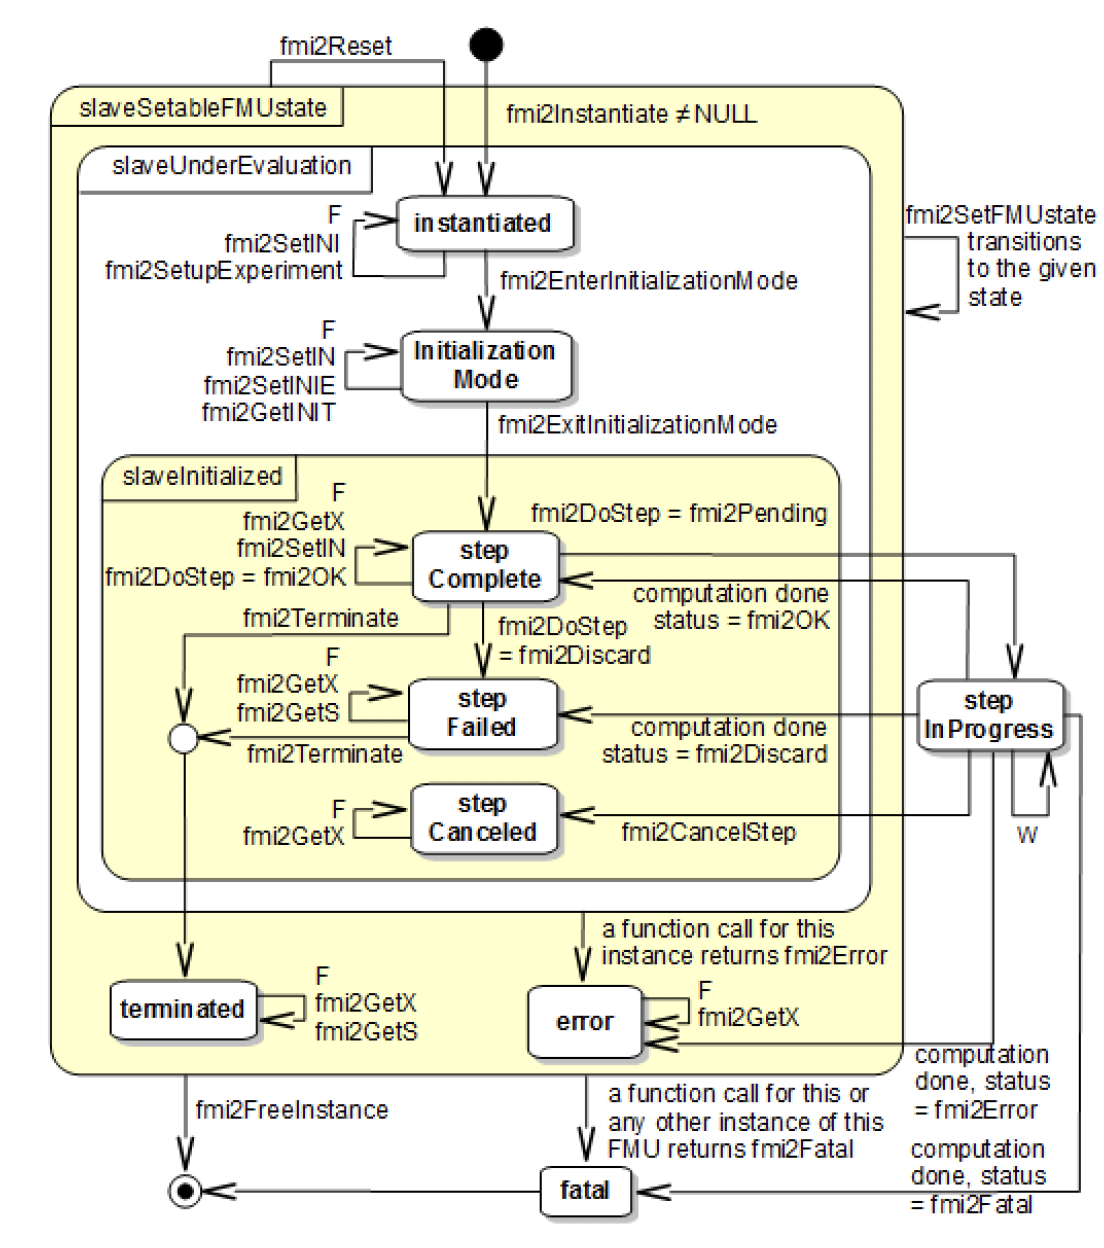
\includegraphics[scale=0.3]{images/Screenshot 2020-09-09 at 08.38.44.png}
\end{figure}
\end{columns}

The goal of the \textbf{Initialization} phase is define all FMU variables and assign them a \textbf{stable} initial value.
\end{frame}

\begin{frame}
\frametitle{But doesn't FMI describe the Initialization of a Co-Simulation?}
FMI describes how to initialize a single FMU and non-connected FMU variables.
The initialization of connected FMUs introduces more challenges (precedence constraints).
\textbf{Interconnected FMU variables require a specific initialization order}.

\begin{figure}
    \centering
    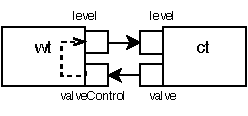
\includegraphics[scale=1.5]{images/ExpansionPlugin-Page-3.pdf}
\end{figure}
Initialization order: $ct.Valve -> wt.valveControl -> wt.level -> ct.level$
\begin{alertblock}{Initialization order} 
    The initialization order is not always trivial! 
\end{alertblock}
\end{frame}

\begin{frame}
\frametitle{Example of a non-trivial Co-Simulation scenario}
A simplified version of a car's suspension system.
\begin{figure}
    \centering
    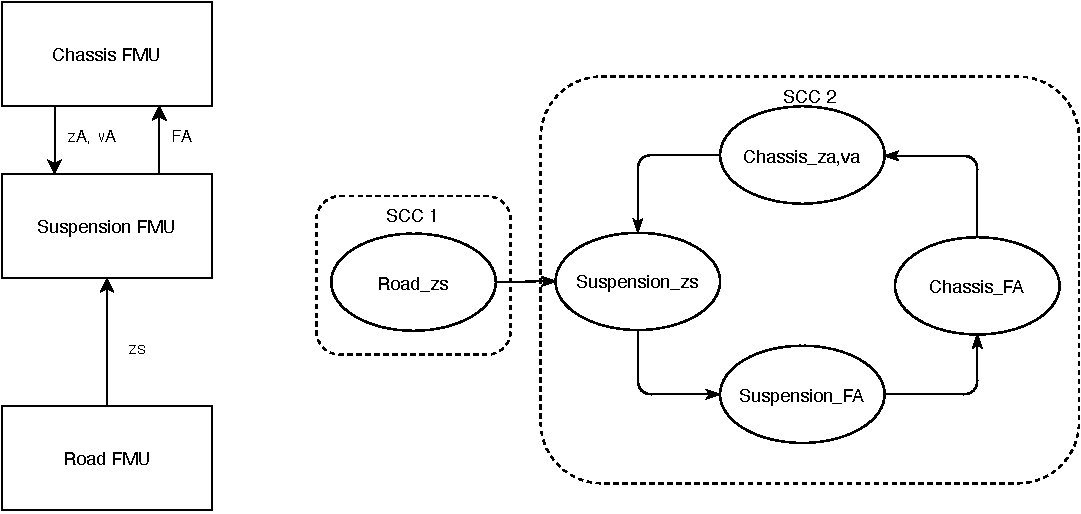
\includegraphics[scale=0.6]{images/quarter_car_SCC.pdf}
    \label{fig:SCC_quarter}
\end{figure}
\end{frame}

\begin{frame}
\frametitle{Non-trivial Co-Simulation scenarios}
\begin{figure}
    \centering
    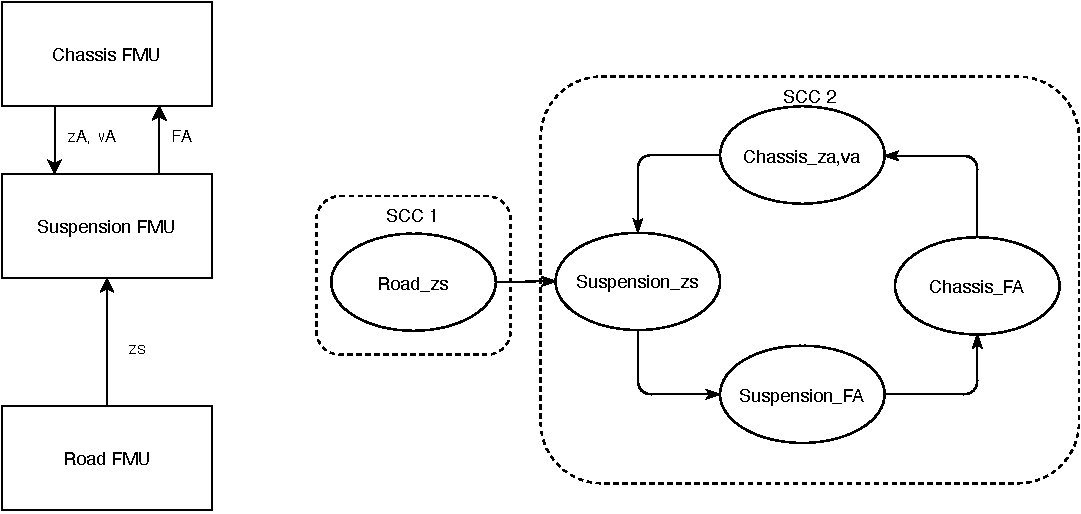
\includegraphics[scale=0.6]{images/quarter_car_SCC.pdf}
    \label{fig:SCC_quarter}
\end{figure}
\begin{itemize}
    \item Algebraic loop - an FMU variable dependence on itself.
\end{itemize}
A loop needs a specific initialization strategy to achieve a correct simulation result!
\textbf{Not} all scenarios containing are stable.
\end{frame}

\begin{frame}[fragile]
\frametitle{Importance of initializing the loops correctly}
\begin{figure}
\centering
\begin{tikzpicture}
    \begin{axis}[
        at={(0,0)},
        width= 10cm,
        height = 7cm,
        ymin=-20,
        ymax=5,
        xmin=0,
        xmax=4.1,
        grid=both,
        grid style={line width=.1pt, draw=gray!10},
        major grid style={line width=.2pt,draw=gray!50},
        axis lines=middle,
        minor tick num =5,
        axis line style={latex-latex},
        ticklabel style={font=\tiny,fill=white},
        minor tick style={draw=none},
        minor grid style={thin,color=black!10},
        ylabel= Car chassis position (cm),
        xlabel= Time (s),
        tick align=outside,
        x label style={at={(axis description cs:0.5,-0.1)},anchor=north, color=blue!50!cyan},
        y label style={at={(axis description cs:-0.1,.5)},rotate=90,anchor=south, color=blue!50!cyan},
        x tick label style={
            /pgf/number format/assume math mode, font=\sf\scriptsize}
        ]
    \addplot [line width=2.5pt, red] table [x= a, y=c, col sep=comma] {incorrect.csv};
    \addplot [y filter/.code={\pgfmathparse{\pgfmathresult*100.}\pgfmathresult}][line width=2.5pt, blue] table [x=a, y=b, col sep=comma] {correct.csv};
\end{axis}
\end{tikzpicture}
    \caption{Simulation results}
    \label{fig:init_state_0_sim}
\end{figure}

\end{frame}

\section{So how to handle these non-trivial scenarios?}
\begin{frame}
\frametitle{So how to handle do the obtain a valid result from a non-trivial scenario?}
\textbf{The characteristics of the co-simulation scenario determines the initialization strategy}
\begin{enumerate}[I]
    \item Identify the characteristics of the co-simulation scenario
    \begin{itemize}
        \item Non-trivial - algebraic loops
        \item Trivial - no algebraic loops
    \end{itemize}
    \item Calculation of a correct initialization order
    \item Initializing the interconnected FMU-variables
\end{enumerate}
\end{frame}

\begin{frame}
\frametitle{Identification of non-trivial co-simulation scenarios}
\begin{itemize}
    \item A graph-based a approach 
    \item The problem is to find all SCCs of the graph
\end{itemize}
\begin{figure}
    \centering
    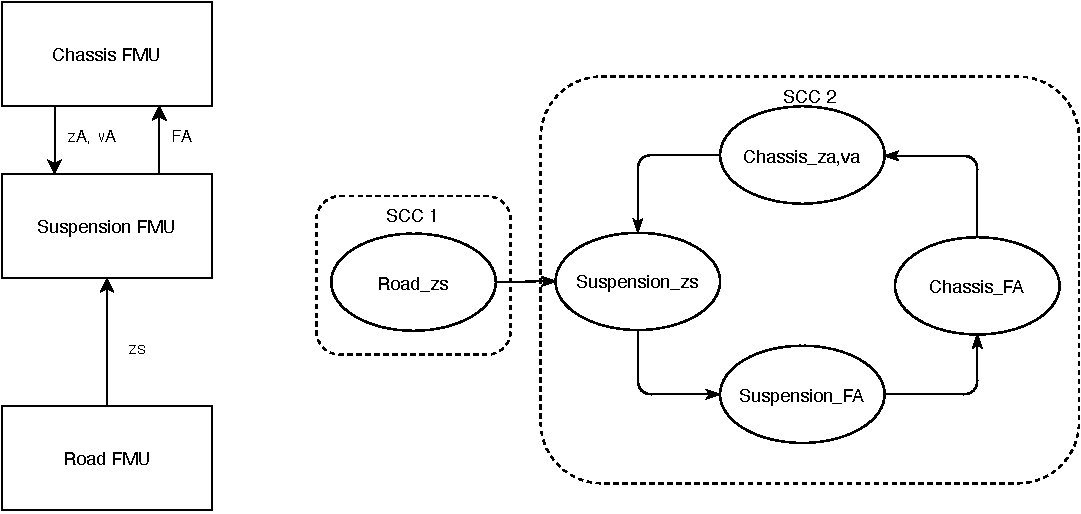
\includegraphics[scale=0.6]{images/quarter_car_SCC.pdf}
    \caption{Generation of a graph of interconnected FMU-variables}
\end{figure}
\end{frame}

\begin{frame}
\frametitle{Calculation of a correct initialization order}
The initialization order is the topological ordering of the SCC of the graph.

\begin{exampleblock}{Optimization of the initialization order}
Variables of a single FMU can be set/read in bulk!
\end{exampleblock}
\end{frame}

\begin{frame}
\frametitle{The initialization strategy for algebraic loops}
    Each loop is initialized using a fixed point iteration strategy until convergence.
    
\begin{figure}
    \centering
    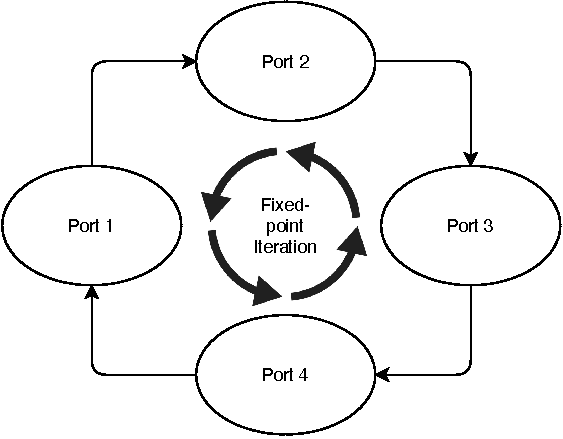
\includegraphics[scale=0.6]{images/ExpansionPlugin-Page-4.pdf}
\end{figure}
    
\begin{alertblock}{Convergence}
    Convergence of a loop is not guaranteed!
\end{alertblock}
    
\end{frame}

\begin{frame}
\frametitle{Checking for convergence}
How do we make sure that our system has reached a stable initial state?
Within a finite number of iterations convergence should  be established.
\begin{figure}
    \centering
    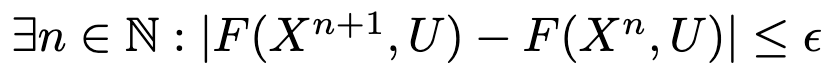
\includegraphics[scale=0.3]{images/Screenshot 2020-09-09 at 20.51.28.png}
\end{figure}

If convergence is not established the co-simulation is dismissed!
\end{frame}

\begin{frame}
\frametitle{The initialization strategy for trivial SCC}
The initialization of trivial SCC is performing the correspondent variable action (set,get) 
    
\end{frame}

\begin{frame}[fragile]
\frametitle{The complete approach}
\begin{figure}
    \centering
    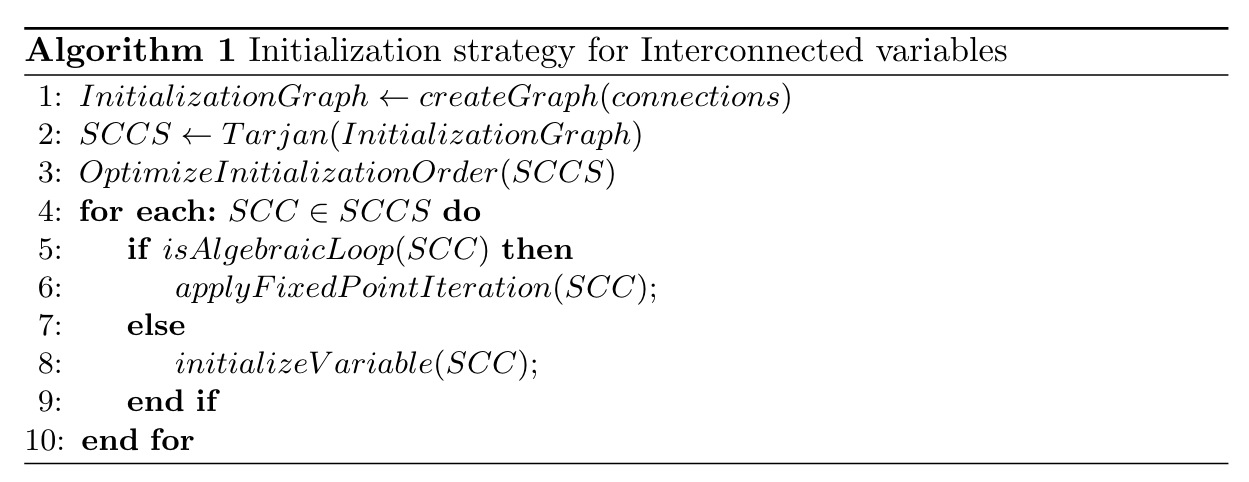
\includegraphics[scale=0.25]{images/Screenshot 2020-09-09 at 09.12.56.png}
\end{figure}

\begin{block}{Remark} 
    The approach is suitable with all well-established master algorithms ()
\end{block}
\end{frame}


\begin{frame}
\frametitle{INTO-CPS Maestro 2}
\begin{itemize}
    \item A part of the INTO-CPS application and a successor of the Maestro.    
    \item Separates the specification (MaBL) of a co-simulation from the simulation.
    \item The specification is typically generated by some plugins
\end{itemize}
\begin{figure}
    \centering
    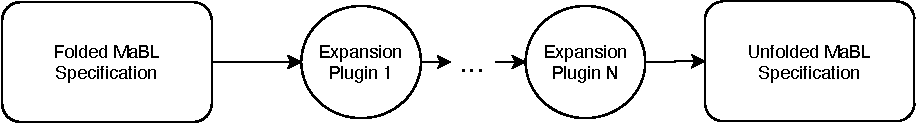
\includegraphics[scale=0.6]{images/ExpansionPlugin-Page-1.pdf}
    \label{fig:my_label}
\end{figure}
\end{frame}


\begin{frame}[fragile]
\frametitle{Maestro Base Language (MaBL)}
The specification of a co-simulation is expressed in MaBL.

\begin{lstlisting}[language=C++]
simulation
import Initializer;
{
FMI2 tankcontroller = load("FMI2", "{8c4e810f-3df3-4a00-8276-176fa3c9f000}", "src/test/resources/watertankcontroller-c.fmu");
...
FMI2Component crtlInstance = tankcontroller.instantiate("crtlInstance", false, false);;
IFmuComponent components[2]={wtInstance,crtlInstance};
expand initialize(components,START_TIME, END_TIME);

SingleWatertank.freeInstance(wtInstance);
}
\end{lstlisting}
\end{frame}


%---------------------------------------------------------
%Changing visivility of the text
\begin{frame}
\frametitle{The implementation of the Approach}
\begin{itemize}
    \item An expansion plugin to Maestro 2
    \item The plugin generates the initialization procedure
    \item The plugin can handle both trivial and non-trivial co-simulation scenarios
    \item The identification of SCCs and topological sorting is done by Tarjan's Algorithm implemented in Scala
\end{itemize}
\end{frame}

\begin{frame}
\frametitle{How do the know the plugin is working?}
\begin{itemize}
    \item The plugin has been verified against the existing \textit{Initializer}
    \item Gomes et al. made an encoding of the rules of order between the FMU operations in Prolog
    \item The calculated initialization order gets checked by the Prolog program
\end{itemize}
\end{frame}


\begin{frame}
\frametitle{Summary - the key takeaways!}
\begin{itemize}
    \item A correct initialization of a co-simulation is crucial to obtain a trustworthy result!
    \item The topological ordering of the interconnected FMU variables  is the initialization order
    \item Co-simulation scenarios containing algebraic loops should be initialized using a fixed-point strategy
    \item The approach is implemented as an expansion plugin to Maestro 2  
\end{itemize}
\end{frame}

\section{Future work}

\begin{frame}
\frametitle{Future work}
\begin{itemize}
    \item Formally verifying the expansion plugin  
    \item Formal verification to guarantee termination of a co-simulation.
\end{itemize}
\end{frame}

\begin{frame}
\frametitle{Questions}
\huge
Thank you!
\end{frame}


\end{document}